\documentclass[noshadow]{LSRslides}
% use class option 'longpres' if you want to use subsections
% use class option 'noshadow' if you want to use blocks without shadow
% beameroptions can be used, e.g. 'handout'

\graphicspath{{pics/}{logos/}}
\addbibresource{ref.bib}
\title{Presentation\\Title}

%%  \addauthor[opt: new line]{name}{opt: affil}
\addauthor{A. Author}{1}
%%  \presenter[opt: new line]{name}{opt: affil} %% underlined
\presenter{M. Mitarbeiter}{2}
%%  \addauthor[opt: new line]{name}{opt: affil}
\addauthor[1]{C. Chef}{3}
\addauthor{C. Chef}{1,2,3}

%%  \addaffiliations[opt: footnote]{line 1}{opt: line 2} 
%% 		if line 2 is omitted line 1 and the following affiliation are combined, see the example
\addaffiliations[1]{Institute for Advanced Study}{}
\addaffiliations[2]{Institute of Automatic Control Engineering}{Technische Universität München}
\addaffiliations[3]{Institute for Whatever}{University of Wolla Wolla}

%% \setprojectlogo[opt: website]{filename}{height}
\setprojectlogo[http://www.cotesys.de]{cotesys}{10mm}

\occasion{International Workshop of Couch Potatoes, Munich}

%% \date{month}{day}{year}
\date{11}{16}{2012}

%% both packs for subfigure 
%%(the subfigure and subfig packages are deprecated and shouldn't be used any more)
\usepackage{caption}
\usepackage{subcaption}
\captionsetup{compatibility=false}
%%%%%%%%%%%%%%%%%%%%%%%%%%%%%%%%%%%%%%%%%%%%%%%%%%%%%%%%%%%%%%%%%%%%%%%%%%%%%%%%
\begin{document}


\begin{frame}
    \titlepage
\end{frame}

\begin{frame}
	\frametitle{Motivation}	
	\begin{columns}[onlytextwidth, T]
	\begin{column}{.5\textwidth}
	Why are we addressing this problem?
			\begin{itemize}
				\item Aaa
				\item Bbb
				\item Ccc
			\end{itemize}
	\end{column}
	\begin{column}{.5\textwidth}
		\only<1>{
\includegraphics[height=4cm]{motivation}}
		\only<2>{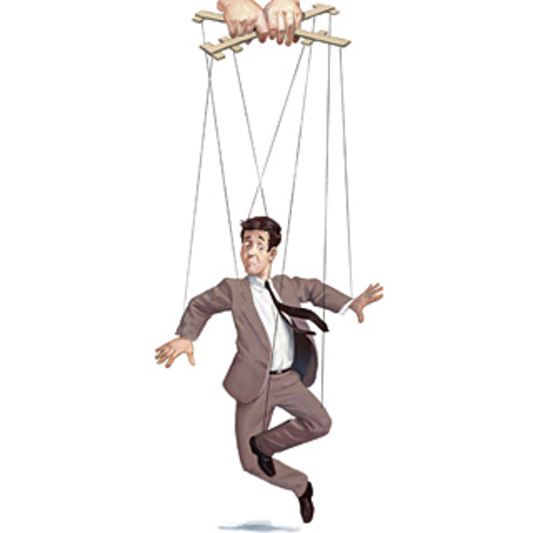
\includegraphics[height=4cm]{control_human}}
	\end{column}
	\end{columns}\vspace{.5cm}
	\uncover<2>{\simpleblock{This is why!}}
\end{frame}

\begin{frame}
    \frametitle{Overview}
	\begin{columns}[onlytextwidth]
	\begin{column}{.4\linewidth}
    \tableofcontents[hidesubsections]%[pausesections]
	\end{column}
	\begin{column}{.6\linewidth}
	\begin{figure}
		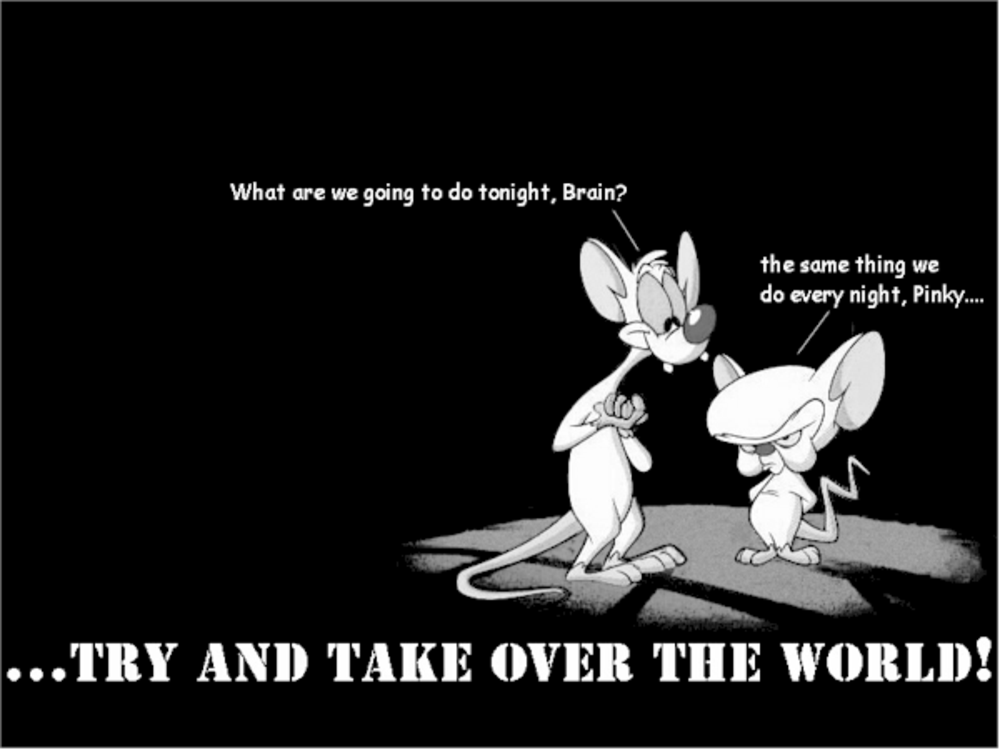
\includegraphics[width=\columnwidth]{pinky}
	\end{figure}
	\end{column}
	\end{columns}
\end{frame}

\section{Introduction}
\begin{frame}
	\frametitle{Problem Formulation}
			\begin{block}{Problem}
				$$x^* = \argmin_{x\in\mathcal{X}} \int J(x,t)\d t$$
			\end{block}
			Challenges:
			\begin{itemize}
				\item Curse of dimensionality
				\item Non-linear model/constraints
				\item No analytical solution
				\item Noisy Measurements
				\item Real-time capability
			\end{itemize}
			\begin{block}{Solution}
				Solve Problem
			\end{block}
\end{frame}

\begin{frame}
	\frametitle{Related Work}
	Normal cite: \cite{buss11}\\
	Bigger cite: \scite{buss11}\\
	Variable number of authors: 
	\begin{itemize}
		\item 2 authors: \varcite{bauer09}{2}
		\item 4 authors: \varcite{bauer09}{4}
	\end{itemize}
\end{frame}

\section[Approach]{Approach Definition}
\begin{frame}
	\frametitle{Approach}
	\dots
\end{frame}

\section{Results}

\begin{frame}
	\frametitle{Results}
	\dots
\end{frame}

\section{Summary}

\begin{frame}
	\frametitle{Summary}
	\dots
\end{frame}

\appendix
%\nocite{buss11}
%\nocite{bauer09}
\begin{frame}
	\frametitle{References}
	%\tiny
	%\bibliographystyle{plain}
	%\bibliography{ref}
	\vspace{\stretch{1}}
	\printbibliography
	\vspace{\stretch{2}}
	This work was supported by:
	\vspace{0.2cm}
	\begin{columns}[onlytextwidth,T]
		\column{.5\textwidth}
		%\begin{figure}
		\centering
		
\includegraphics[height=1cm]{iuro}\\
		\href{http://www.iuro-project.eu}{\texttt{www.iuro-project.eu}}
		%\end{figure}
		\column{.5\textwidth}
		%\begin{figure}
		\centering
		
\includegraphics[height=1cm]{cotesys}\\
		%\end{figure}
		\url{www.cotesys.org}
	\end{columns}
	\vspace{\stretch{1}}
\end{frame}

\end{document}
